\documentclass[11pt]{article}
\usepackage[margin=0.88in]{geometry}
\usepackage{amsmath,amssymb,booktabs,enumitem,float,graphicx,hyperref,microtype,tabularx,xcolor,xspace}
\hypersetup{colorlinks=true,linkcolor=blue!55!black,citecolor=blue!55!black,urlcolor=blue!55!black}
\newcommand{\pra}{\textsc{PRA}\xspace}
\newcommand{\qk}{\textsc{QK}\xspace}
\newcommand{\kv}{\textsc{K/V}\xspace}
\newcommand{\hotpot}{HotpotQA\xspace}
\newcommand{\qasper}{QASPER\xspace}
\setlength{\emergencystretch}{3em}

\title{Distilling Native Query--Key Responses into Compact Memory Landmarks}
\author{Jorge Sim\~ao\\EInnovator R\&D -- Center for the Sciences of Computation, Cognition, and Complexity}
\date{August 2026}

\begin{document}
\maketitle

\begin{abstract}
Progressive Retrieval Attention (\pra) uses compact routing gists to choose long-memory chunks, then materializes the selected chunks' unchanged native key/value (\kv) states. Mean gists are inexpensive but erase sparse token-level address signals. We ask whether one to eight actual pretrained keys can preserve a frozen transformer's full chunk-response surface. Validation uses 16 identity-disjoint \hotpot/\qasper questions; testing uses the frozen 32-question Paper 2.5/2.6 cohort, a fixed four-chunk materialization budget, and five seeds. A key-only selector improves \qasper over the Paper 2.6 semantic gist but recovers only 40.5\% of oracle response-preservation gain. We then cross low-rank query conditioning $r\in\{8,16,32\}$, $m\in\{4,8\}$ landmarks, and four losses: oracle imitation, evidence-listwise ranking, ranking plus response distillation, and a top-four-boundary loss. The prespecified combined $r=16,m=4$ controller raises \hotpot recall from 0.1235 to 0.1667, paired difference 0.0432 with 95\% interval $[-0.0112,0.0970]$, but falls below strong lexical channels and reduces \qasper recall to 0.0574. Exploratorily, decision-aware $r=32,m=8$ reaches \qasper recall 0.1718, close to exact routing at 0.1776; its five seed means span 0.1639--0.1796, but paired intervals against exact and the key-only selector include zero. Query conditioning raises maximum oracle-gain recovery only to 47.3\%, below the prespecified 80\% gate. Native response compression therefore does not yield one universal controller: evidence utility depends jointly on dataset, landmark budget, and training objective.
\end{abstract}

\section{Introduction}
\pra separates \emph{routing} from \emph{reading}. A small summary chooses memory chunks; only the chosen chunks contribute their original token \kv to attention. The separation preserves pretrained values and bounds active memory, but it makes routing-summary quality consequential. One mean vector per chunk is attractive because it is deterministic, cacheable, and cheap. It is also a severe compression: a sparse key that responds strongly to a future query can disappear inside 31 unrelated tokens.

Earlier work already tested natural repairs. Multi-gist, prototype, $k$-means, SOM, local-gist, native-\qk closure, lexical, and graph-query variants sometimes helped a dataset or controlled fixture, but did not establish a uniform natural frontier. Those methods mainly organize semantic or local geometry. This paper asks a different question: can a compact native-key set preserve the \emph{response surface} that the frozen attention layer assigns to the full chunk?

The distinction matters. A key is useful because of how plausible queries address it, not because it reconstructs the mean of its neighbors or reads well as text. We therefore use full token-level keys as a teacher, measure ranking preservation directly, and keep the downstream materialization budget fixed. The study is gated. We first verify inherited Paper 2.6 rows, then test whether the teacher is meaningful, then ask whether a query-aware oracle has headroom. A learned selector is permitted only after those checks; more expressive off-manifold slots and recurrent memory remain closed if it fails.

The contributions are:
\begin{enumerate}[leftmargin=*]
  \item a tensor-native definition of chunk response distillation under grouped-query attention, with max, top-$r$, log-sum-exp, and attention-mass teachers;
  \item matched native-key controllers, response metrics, routing metrics, changed-selection audits, and synchronized CUDA cost measurements;
  \item a controlled 32--256-token suite and a frozen natural evaluation aligned with the Paper 2.5/2.6 32-token chunk and four-chunk budget;
  \item a measured boundary: oracle landmarks show natural QASPER headroom, while a 321-parameter key-only selector recovers too little of that headroom to pass deployment gates;
  \item a 120-controller query-conditioned sweep separating a prespecified primary result from test-selected exploratory findings and showing that response preservation, evidence ranking, and dataset utility are not interchangeable.
\end{enumerate}

\section{Native response distillation}
\subsection{Full-key teacher}
Let chunk $C$ contain pre-RoPE native keys $K_C\in\mathbb{R}^{n\times H_{kv}\times d_h}$ and let a frozen decoder produce query heads $q\in\mathbb{R}^{H_q\times d_h}$. The grouped-query map $g(h)$ assigns each query head to its native key head. Scaled token responses are
\begin{equation}
  a_{i,h}(q,C)=\frac{q_h^\top k_{i,g(h)}}{\sqrt{d_h}}.
\end{equation}
The teacher reduces tokens per head and then averages heads:
\begin{equation}
  S^*(q,C)=\frac{1}{H_q}\sum_h F\left(a_{1,h},\ldots,a_{n,h}\right).
\end{equation}
We validate four reductions: maximum, top-$r$ mean, length-normalized log-sum-exp, and a softmax attention-mass proxy. Validation selects top-four mean with $r=4$. This selection occurs before test evaluation and is frozen for every controller.

For compact landmarks $G(C)=\{\hat{k}_1,\ldots,\hat{k}_m\}$, the estimate $\hat S(q,C)$ applies the same $F$ and grouped-head mapping. The primary target is not $\|K_C-\hat K_C\|$. It is agreement between $S^*$ and $\hat S$ over candidate chunks: score error, rank correlation, teacher top-$k$ overlap, and KL divergence between softmax-normalized chunk distributions.

\subsection{Controllers}
All deployable landmark outputs are actual pretrained keys. Mean is the only synthetic control.
\begin{description}[leftmargin=2.4cm,style=nextline]
\item[Mean] Average valid keys independently in each native key head, yielding one key per chunk.
\item[Last and random] Retain the final $m$ valid keys or a deterministic random subset.
\item[Farthest-first] Flatten native heads per token and greedily retain cosine-diverse keys.
\item[Greedy oracle] Add the token that most reduces full-response squared error. It sees the evaluation query and is explicitly non-deployable.
\item[Learned selector] Score each token from overall key norm, mean head norm, head-norm variation, cosine to the chunk centroid, local key change, forward/reverse position, and validity. A two-layer MLP, $8\rightarrow32\rightarrow1$, has 321 parameters. Hard top-$m$ is used at inference.
\end{description}

Oracle selections for $m=8$ supervise the learned model. Five seeds train for 400 AdamW steps on 16 validation identities. The backbone, native projections, tokenizer, and all natural test identities remain frozen. The selector receives no question vector, evidence label, dataset identifier, lexical feature, or chunk-level answer supervision at inference.

\subsection{Query-conditioned continuation}
The continuation addresses the key-only selector's missing information need without changing native keys. Let $f_i\in\mathbb{R}^8$ be token $i$'s normalized key-only features and let $\bar q\in\mathbb{R}^{H_qd_h}$ be the flattened, RMS-scaled native query. The selector logit is
\begin{equation}
  z_i=\operatorname{MLP}(f_i)+\frac{(W_q\bar q)^\top(W_ff_i)}{\sqrt r},
\end{equation}
where $r\in\{8,16,32\}$. The resulting models have 16,769, 33,217, and 66,113 parameters. Hard top-$m$ selects actual native keys at inference.

Training uses a piecewise-differentiable surrogate only to move selector logits. Within each chunk, the hard top-$m$ support is retained while a softmax over its logits weights scalar native token responses. This gives a chunk surrogate $\widetilde S(q,C)$. Final evaluation discards the surrogate, gathers hard-selected keys, and recomputes $\hat S(q,C)$ with the exact grouped-query native-\qk function.

Four objectives are prespecified. \emph{Oracle imitation} applies token-level weighted binary cross-entropy to greedy response-preserving selections. \emph{Listwise} minimizes cross-entropy from the chunk softmax to a uniform distribution over evidence chunks. \emph{Combined} adds $\mathrm{KL}(\operatorname{softmax}S^*\|\operatorname{softmax}\widetilde S)$ to listwise ranking. \emph{Decision-aware} adds pairwise softplus penalties between evidence chunks and non-evidence chunks nearest the fourth-place routing threshold. We cross all four objectives with both landmark counts, all three ranks, and five seeds: 120 controllers, each trained for 300 AdamW steps on validation only. Combined $r=16,m=4$ is the prespecified primary configuration; every other test comparison is reported without replacing it.

\subsection{Matched materialization}
The intervention changes only routing summaries. Candidate units are the same 32-token local chunks. Every method requests four chunks, so it materializes approximately 128 native \kv tokens: 126.1 on \hotpot because of short final chunks and 128.0 on \qasper. Active memory fractions are 8.8\% and 3.3\%, respectively. Values are never compressed, projected, or synthesized.

\section{Protocol}
\subsection{Frozen natural cohort}
We reuse Qwen3-0.6B revision \texttt{c1899de2}, layer 27, 16 query heads, eight \kv heads, and head width 128. Source blocks are encoded in bounded 256-token calls, then divided into 32-token routing chunks without local re-encoding. Pre-RoPE keys and attention-input query states preserve token spans and evidence masks. The query state is projected through the unchanged native \texttt{q\_proj} and \texttt{q\_norm}.

Validation contains eight \hotpot and eight \qasper identities. Test contains 16 of each, matching the frozen Paper 2.5/2.6 identities and excluding validation identities. Feature tensors are 329 MB and 621 MB, respectively; manifests record SHA-256 hashes. Paper 2.6's 224 test rows are re-aggregated exactly at G0. Paper 2.5's 256-token-parent, 20\%-budget rows are retained only as historical context because their candidate unit and budget are not numerically matched.

\subsection{Controlled suite}
Twenty synthetic cases cross chunk sizes $n\in\{32,64,128,256\}$. Each case has 16 candidate chunks. An evidence chunk contains sparse query-aligned native keys while a distractor has a coherent but weaker mean. This tests whether full-key and landmark controllers preserve a sparse address that averaging can hide. The suite is a mechanism check, not evidence for natural language performance.

\subsection{Metrics and uncertainty}
Native preservation metrics are MAE, RMSE, Spearman $\rho$, Kendall $\tau$, KL divergence, and teacher top-$k$ overlap for $k\in\{1,2,4,8\}$. Routing metrics are evidence recall and precision, any-evidence recall, contiguous evidence-group completion, exact selected identity, MRR, active memory fraction, evidence-normalized overhead, materialized tokens, native dots, and wall time. Five-thousand-draw paired bootstrap intervals resample identities. Selector seeds are averaged within identity before comparisons with deterministic baselines.

The prespecified gates are:
\begin{itemize}[leftmargin=*]
  \item G0: inherited Paper 2.6 aggregation parity;
  \item G1: full-K beats mean on controlled recall and at least one natural dataset;
  \item G2: greedy $m\leq8$ improves teacher top-four overlap and at least one natural recall result without changing materialized \kv;
  \item G3: the learned selector recovers at least 80\% of oracle gain, improves recall or completion on one natural dataset, and regresses by less than 0.02 elsewhere;
  \item G4/G5: synthetic slots and streaming memory run only after G3 passes.
\end{itemize}

\section{Results}
\subsection{Teacher sanity and oracle headroom}
G0 passes with zero mismatches across 224 inherited rows. Validation selects top-four mean across query heads: its validation evidence recall is 0.1387 versus 0.1255 for the corresponding mean-key control. Max, log-sum-exp, and attention-mass teachers do not beat that control on validation.

G1 also passes, narrowly on natural data. Full-K recall is 1.000 versus 0.950 for mean in the controlled suite. On held-out \hotpot it is 0.1240 versus 0.1235; on \qasper it is 0.1252 versus 0.0976. The natural teacher is therefore not a strong retrieval oracle by itself. It provides a modest QASPER signal and essentially no Hotpot gain.

\begin{table}[t]
\centering
\caption{Held-out four-chunk routing. Learned rows average five seeds. Oracle rows use the test query and are non-deployable. Values are evidence recall; parentheses give teacher top-four overlap.}
\label{tab:natural}
\begin{tabular}{lcc}
\toprule
Method & \hotpot & \qasper \\
\midrule
Mean key, $m=1$ & 0.124 (0.594) & 0.098 (0.516) \\
Full-K teacher & 0.124 (1.000) & 0.125 (1.000) \\
Farthest-first, $m=2$ & 0.142 (0.734) & 0.130 (0.422) \\
Greedy oracle, $m=4$ & 0.145 (0.922) & \textbf{0.178} (0.703) \\
Greedy oracle, $m=8$ & 0.124 (0.984) & 0.136 (0.812) \\
Learned selector, $m=4$ & 0.122 (0.741) & 0.083 (0.422) \\
Learned selector, $m=8$ & 0.124 (0.834) & 0.139 (0.553) \\
\bottomrule
\end{tabular}
\end{table}

G2 passes. Relative to mean, greedy $m=8$ improves aggregate teacher top-four overlap by 0.3438. Recall is not monotone in $m$: $m=4$ is best, improving \hotpot by 0.0219 and \qasper by 0.0802. The paired intervals, $[-0.0313,0.0750]$ and $[-0.0142,0.2233]$, both include zero. Oracle landmarks therefore establish response-preservation headroom and a promising QASPER direction, not a statistically resolved natural retrieval gain.

\begin{figure}[t]
\centering
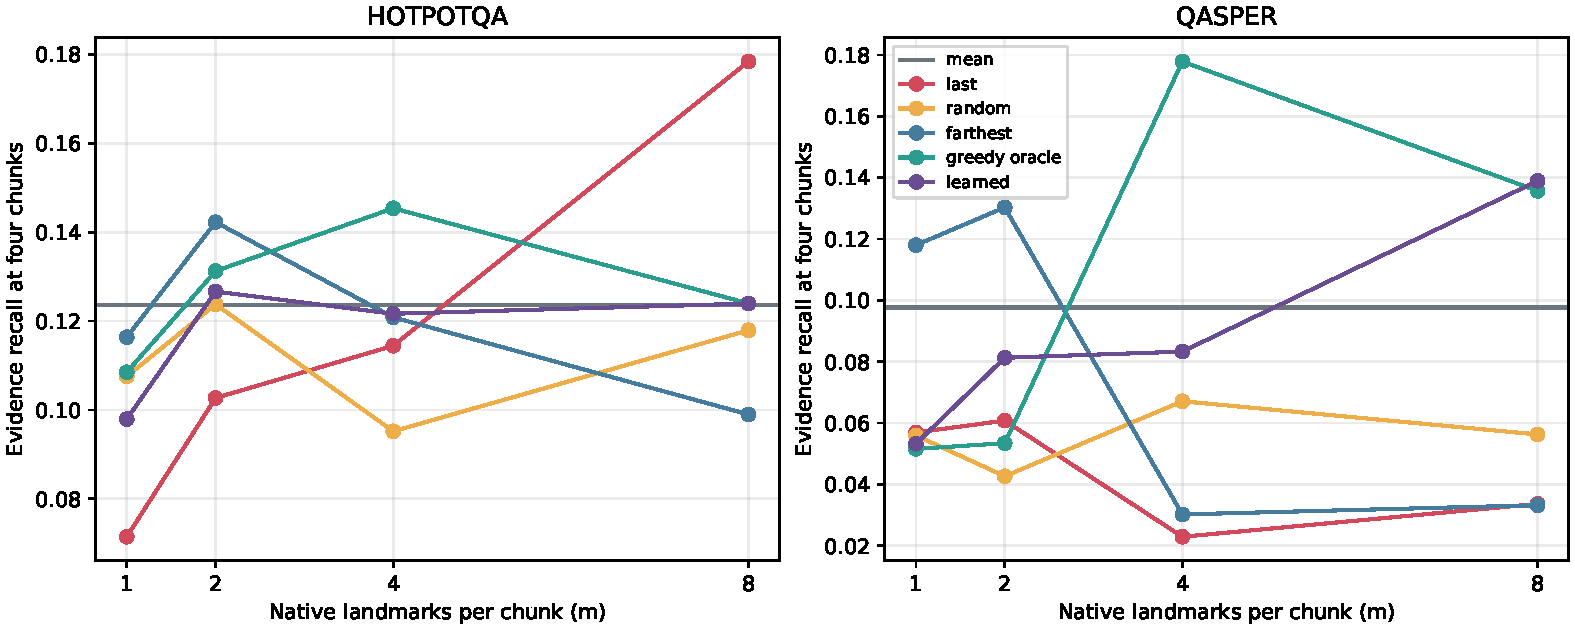
\includegraphics[width=\linewidth]{../shared/results/paper2_8_qk_compression/natural_retrieval_by_dataset.pdf}
\caption{Natural evidence recall under the matched four-chunk materialization budget. The dataset-separated view exposes the Hotpot/QASPER asymmetry.}
\label{fig:natural}
\end{figure}

\subsection{Learned selector: useful direction, failed gate}
The learned selector does not recover the oracle. At $m=8$, it captures 40.5\% of the oracle teacher-overlap gain, below the 80\% threshold. Its \hotpot recall delta over the QK mean is $+0.0004$ with interval $[-0.0573,0.0533]$. Its \qasper delta is $+0.0413$ with interval $[-0.0589,0.1670]$. G3 therefore fails and G4/G5 do not run.

Seed variation is material. \hotpot $m=8$ recall ranges from 0.1173 to 0.1298. \qasper ranges from 0.0478 to 0.1821; four seeds are at or above 0.119, while seed 37 collapses. Teacher top-four overlap is more stable than evidence recall, showing that response imitation and evidence utility are related but not interchangeable.

\subsection{Query conditioning: objective-dependent utility}
The prespecified combined $r=16,m=4$ controller improves \hotpot recall from the full-key teacher's 0.1235 to 0.1667, a paired difference of 0.0432 with interval $[-0.0112,0.0970]$. It also improves over the key-only $m=8$ selector by 0.0427, interval $[-0.0015,0.0907]$. This is the best \hotpot result in the 24-configuration continuation, but remains below BM25, exact, and hybrid routing. The same controller reaches only 0.0574 on \qasper, 0.0402 below the mean-key control and 0.1202 below exact routing. Query conditioning therefore does not produce a dataset-uniform primary result.

The test-selected exploratory result is more encouraging but is not confirmatory. Decision-aware $r=32,m=8$ reaches 0.1718 \qasper recall, compared with 0.1776 for Paper 2.6 exact routing, 0.1389 for the key-only selector, and 0.0976 for the mean key. Its paired differences are $-0.0059$ against exact, interval $[-0.1831,0.2049]$, and $+0.0328$ against key-only, interval $[-0.0292,0.1073]$. Five seed means span 0.1639--0.1796. The narrow seed range shows optimization stability for this configuration; the wide identity-bootstrap intervals show that 16 test questions per dataset are still too few to resolve comparative retrieval utility.

\begin{table}[t]
\centering
\caption{Matched four-chunk evidence recall. ``Primary'' was fixed before test evaluation. ``Exploratory'' is the best \qasper row selected after inspecting the 24-configuration test matrix.}
\label{tab:query-conditioned}
\begin{tabular}{lcc}
\toprule
Method & \hotpot & \qasper \\
\midrule
QK mean & 0.124 & 0.098 \\
Key-only learned, $m=8$ & 0.124 & 0.139 \\
Paper 2.6 BM25 & 0.398 & 0.042 \\
Paper 2.6 exact & 0.287 & 0.178 \\
Paper 2.6 hybrid & 0.279 & 0.081 \\
Primary combined, $r=16,m=4$ & \textbf{0.167} & 0.057 \\
Exploratory decision-aware, $r=32,m=8$ & 0.143 & \textbf{0.172} \\
\bottomrule
\end{tabular}
\end{table}

\begin{figure}[H]
\centering
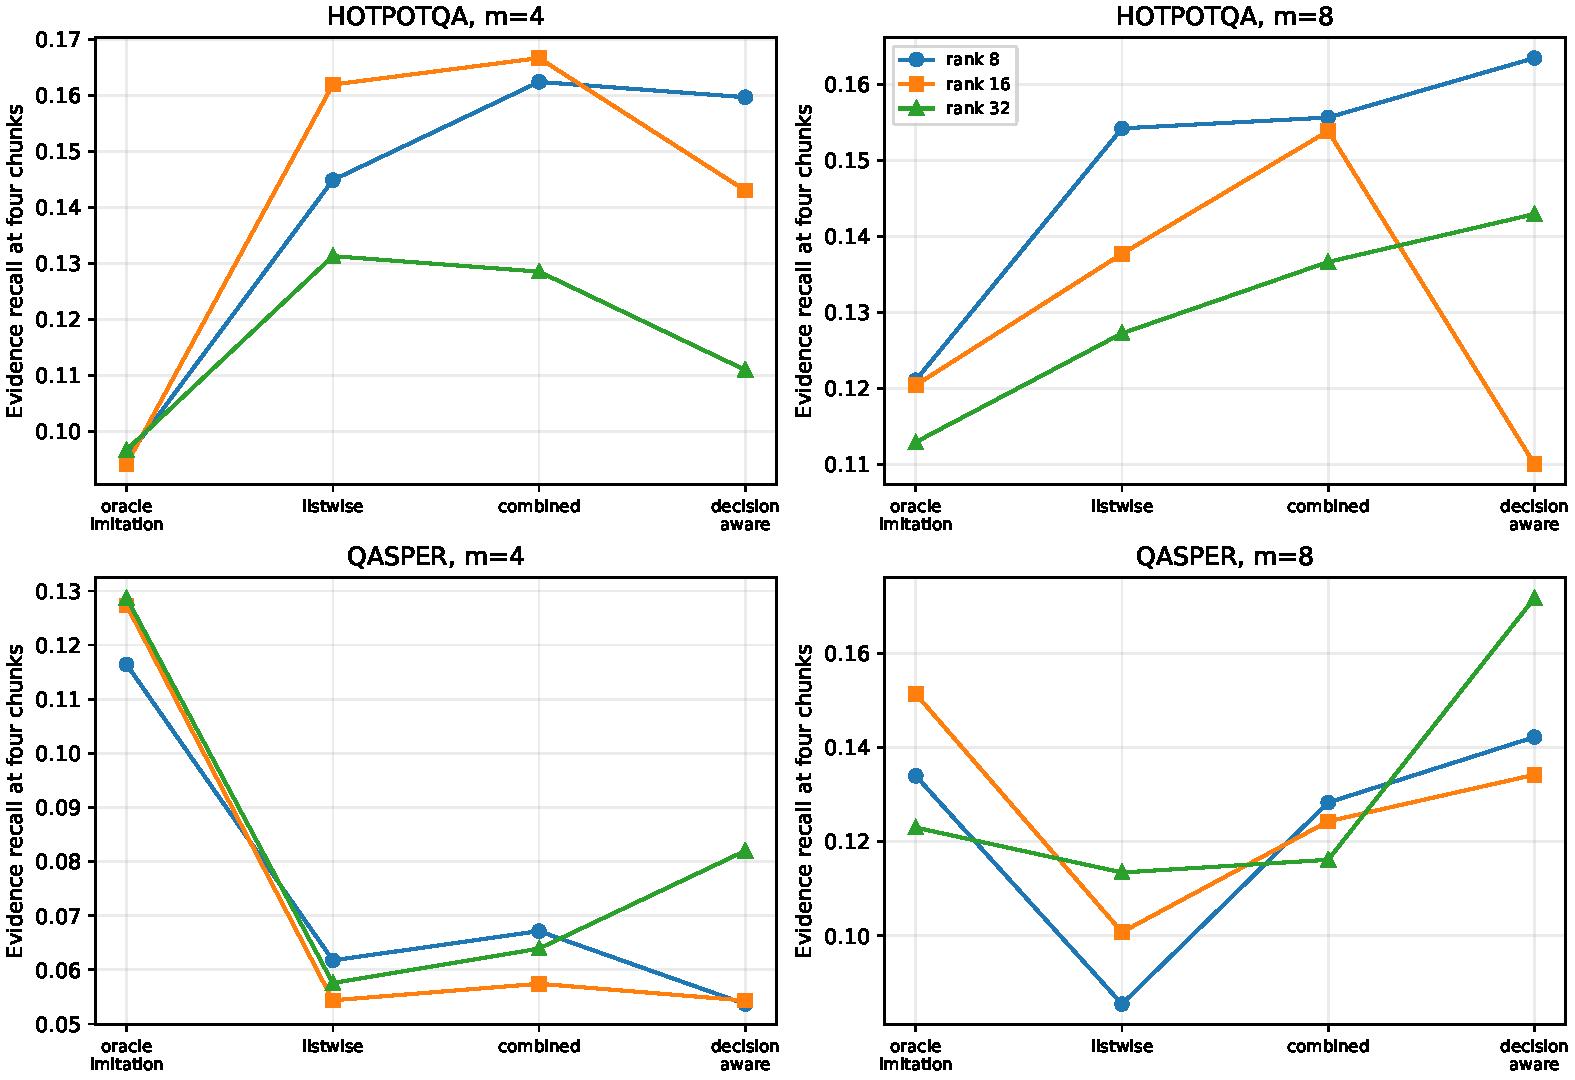
\includegraphics[width=0.98\linewidth]{../shared/results/paper2_8_qk_compression/query_conditioned/objective_rank_recall.pdf}
\caption{Evidence recall across objective, low-rank width, and landmark count. Objective choice changes both the level and the dataset direction; additional rank or landmarks are not monotonically beneficial. Points average five selector seeds.}
\label{fig:query-conditioned}
\end{figure}

Response preservation does not select the same controller as retrieval utility. Oracle-imitation $r=32,m=8$ gives the best aggregate teacher top-four overlap, 0.717 versus 0.555 for mean and 0.898 for greedy oracle, recovering 47.3\% of oracle gain. Yet across the 24 configurations, teacher overlap and evidence recall correlate negatively on \hotpot ($r=-0.665$) and positively on \qasper ($r=0.682$). These descriptive correlations do not establish causality, but they make the failure mode visible: matching a frozen layer's response can preserve preferences that are not evidence-bearing.

\begin{figure}[H]
\centering
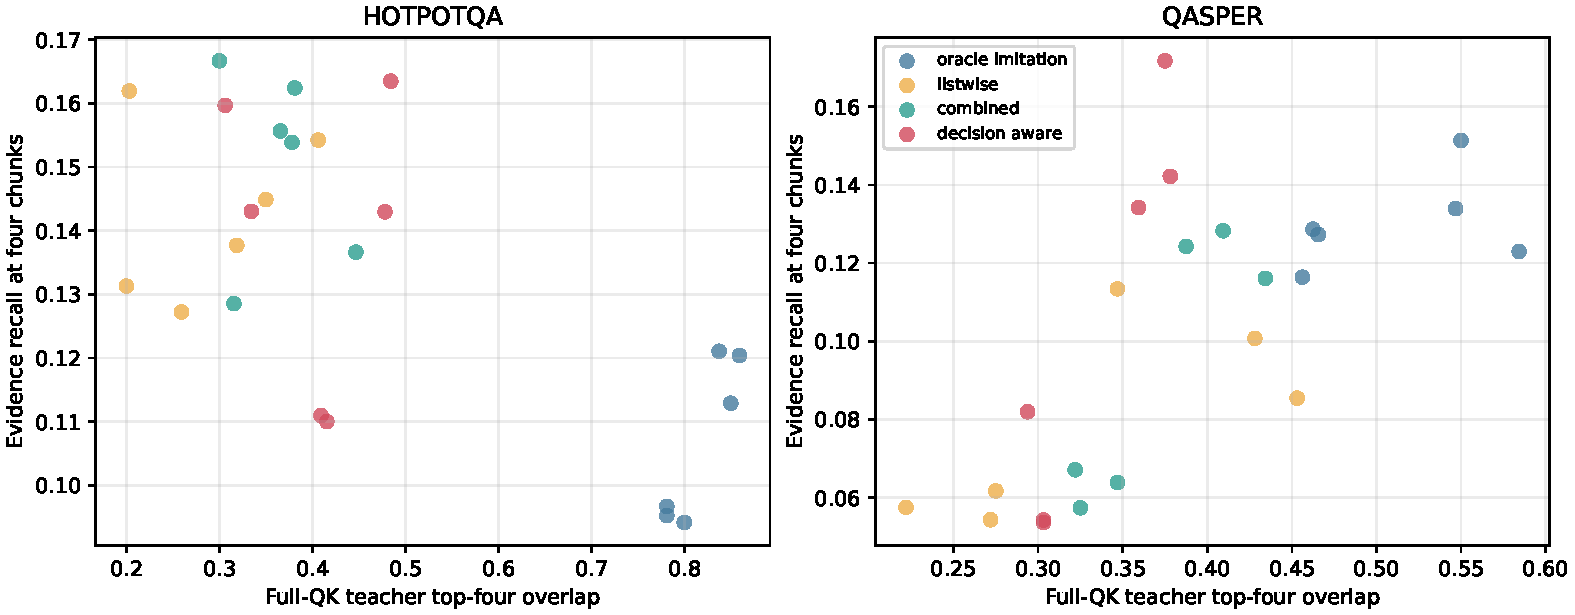
\includegraphics[width=0.82\linewidth]{../shared/results/paper2_8_qk_compression/query_conditioned/recall_vs_preservation.pdf}
\caption{Response preservation versus evidence recall for all 24 query-conditioned configurations. The opposing dataset trends explain why the highest-fidelity compressor is not a universal retrieval controller.}
\label{fig:preservation-recall}
\end{figure}

The primary selector has 33,217 parameters and trains in 36.2 seconds per seed; the exploratory selector has 66,113 parameters and trains in 50.2 seconds per seed on the GTX 950M. Synchronized selector-plus-top-$m$ latency is 42.6/117.0 ms for the primary and 42.9/120.5 ms for the exploratory controller on \hotpot/\qasper. These continuation timings exclude compact-key QK scoring and materialization, so they are component measurements rather than direct replacements for Table~\ref{tab:cost}.

\subsection{Comparison with Paper 2.6}
Figure~\ref{fig:paper26} compares the same frozen identities and four-chunk budget. Learned QK $m=8$ is not a new overall frontier. On \hotpot its 0.124 recall is below Paper 2.6 BM25 (0.398), exact (0.287), and iterative hybrid (0.279), with paired intervals excluding zero against all three. On \qasper it reaches 0.139: above Paper 2.6's semantic gist (0.038) by 0.1010, with paired interval $[0.00004,0.2270]$; above iterative hybrid (0.081) by 0.0579, interval $[-0.0610,0.1974]$; and below exact routing (0.178) by 0.0387, interval $[-0.1951,0.1334]$. The positive, defensible claim is dataset-specific: native response distillation improves the old QASPER semantic-gist baseline, but does not displace lexical exact matching and does not transfer to Hotpot.

\begin{figure}[H]
\centering
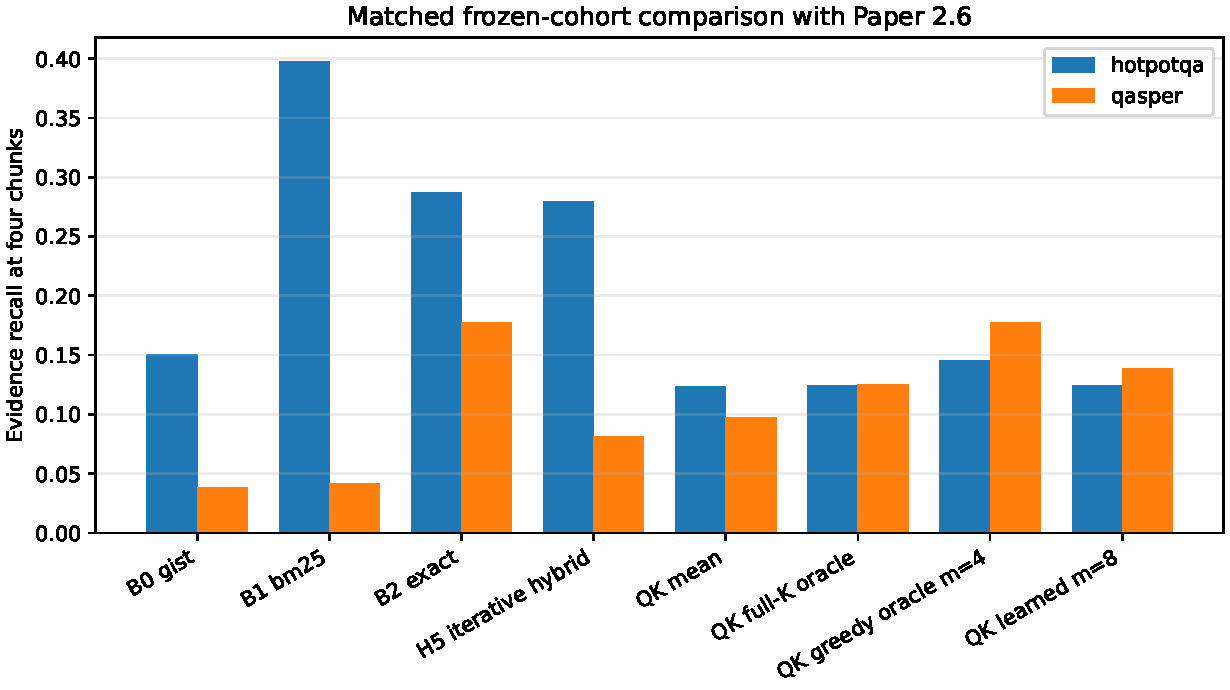
\includegraphics[width=0.94\linewidth]{../shared/results/paper2_8_qk_compression/paper2_6_matched_comparison.pdf}
\caption{Matched Paper 2.6 comparison. Full-K and greedy rows are non-deployable upper bounds. Learned QK is competitive on QASPER but not Hotpot.}
\label{fig:paper26}
\end{figure}

Paper 2.5's native-\qk closure used 256-token parents and a 20\% final-parent budget. At that setting, its top-four native closure reached chain completion 0.125 on \hotpot and 0.875 on \qasper, compared with one-shot parent values 0.138 and 0.938. Those rows concern associative successor discovery, not one-shot 32-token ranking. We preserve them as historical controls but do not pool their metrics with Table~\ref{tab:natural}.

\subsection{Cost}
The synchronized CUDA audit includes uncached controller construction, compact-key gathering, and QK scoring. Table~\ref{tab:cost} reports means over all 32 test identities on an NVIDIA GTX 950M. Absolute times are hardware-specific; the ordering and native-dot counts expose algorithmic differences.

\begin{table}[t]
\centering
\caption{End-to-end routing-controller cost at $m=8$. Mean uses $m=1$. The full-K row performs no selection.}
\label{tab:cost}
\begin{tabular}{lrrrr}
\toprule
 & \multicolumn{2}{c}{\hotpot (50.1 chunks)} & \multicolumn{2}{c}{\qasper (142.6 chunks)} \\
Method & ms & native dots & ms & native dots \\
\midrule
Mean & 6.1 & 802 & 10.7 & 2,282 \\
Full-K & 25.9 & 24,898 & 34.1 & 70,853 \\
Farthest-first & 463.1 & 6,416 & 1,308.4 & 18,256 \\
Greedy oracle & 24,367.6 & 6,416 & 70,376.0 & 18,256 \\
Learned selector & 102.8 & 6,416 & 259.9 & 18,256 \\
\bottomrule
\end{tabular}
\end{table}

The learned selector is 4.5--5.0 times faster than farthest-first and about 237--271 times faster than the top-$r$ greedy oracle, but 16.9--24.4 times slower than mean on this unoptimized Python/CUDA path. Greedy cost is dominated by query-aware candidate search, not compressed scoring. The quality CSV's \texttt{compression\_ms} field times compact assembly after indices are cached; Table~\ref{tab:cost} instead uses the separate synchronized uncached audit.

\begin{figure}[H]
\centering
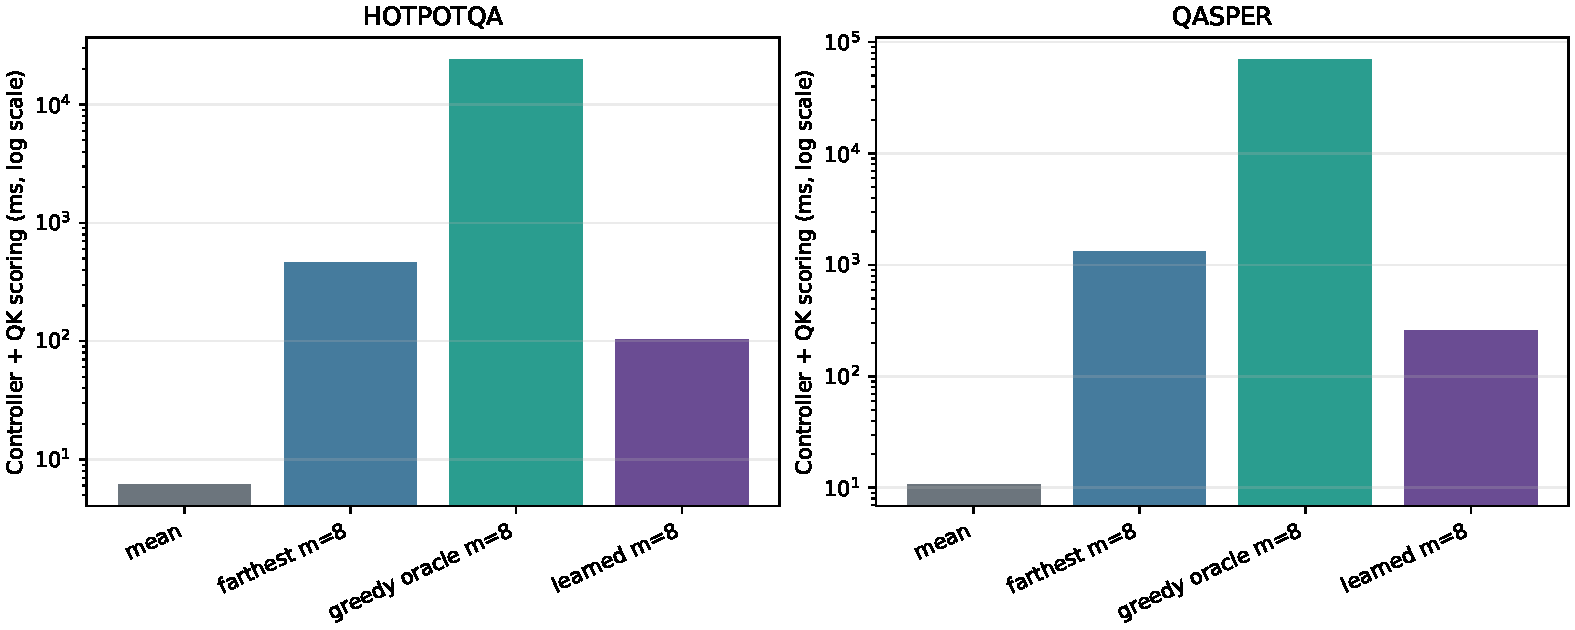
\includegraphics[width=0.84\linewidth]{../shared/results/paper2_8_qk_compression/controller_cost.pdf}
\caption{Controller construction plus QK scoring on a log scale. The oracle is a feasibility instrument, not a serving method.}
\label{fig:cost}
\end{figure}

\subsection{Gate summary}
\begin{table}[H]
\centering
\caption{Prespecified decisions. The sequence stops at G3.}
\begin{tabularx}{\linewidth}{llX}
\toprule
Gate & Status & Evidence \\
\midrule
G0 & Pass & 224 inherited Paper 2.6 rows reproduce with zero aggregate mismatches. \\
G1 & Pass & Controlled recall 1.00 vs. 0.95; full-K improves QASPER mean-key recall by 0.0276. \\
G2 & Pass & Greedy $m=8$ top-four overlap $+0.3438$; greedy $m=4$ QASPER recall $+0.0802$. \\
G3 & Fail & Key-only recovers 40.5\%; the best query-conditioned oracle-imitation row recovers 47.3\%. Both are below 80\%. \\
G4 & Closed & Synthetic off-manifold slots require G3. \\
G5 & Closed & Streaming recurrent memory requires an offline compressor pass. \\
\bottomrule
\end{tabularx}
\end{table}

\section{What the result means}
Three observations explain the outcome.

First, a full-key teacher is not automatically an evidence oracle. Native attention keys encode many functions besides document retrieval, and a question's final layer-27 query can respond to syntactic, discourse, and answer-format features. Top-four mean is the best validated reduction here, but its natural advantage over a mean key is small.

Second, response approximation and top-four selection are different objectives. Greedy $m=8$ nearly reproduces the teacher ranking on \hotpot yet does not improve recall. On \qasper, $m=4$ retrieves more evidence than $m=8$ despite lower teacher overlap. Additional landmarks can faithfully restore teacher preferences that are irrelevant or harmful to evidence selection. A future objective should combine teacher distillation with validation-only ranking calibration rather than treating the teacher as ground truth.

Third, query conditioning addresses the key-only selector's missing information need, but does not remove objective mismatch. The combined loss gives the best \hotpot result and a poor \qasper result; decision-aware training gives the best \qasper result; oracle imitation gives the best response preservation. Capacity alone is not the explanation: increasing rank and landmark count is not monotone, and a controller can reproduce the teacher while retrieving less evidence.

The next justified experiment is a fresh, larger, identity-disjoint confirmation in which dataset-specific objective selection occurs entirely on validation. It should prespecify combined $r=16,m=4$ for \hotpot and decision-aware $r=32,m=8$ for \qasper, retain BM25/exact/hybrid controls, and include downstream native-\kv answer generation. Synthetic slots and recurrent state remain premature because no native-key selector closes the response-recovery gate.

\section{Relation to prior PRA results}
Paper 1 established mean-gist routing and selected native \kv. Paper 2.5 tested iterative associative closure and showed that local/native propagation can solve controlled bridges without yielding a uniform natural gain. Paper 2.6 demonstrated strong channel asymmetry: lexical evidence is particularly effective for Hotpot and exact matching for QASPER. Paper 2.7 moved structure discovery to the query side and found that better natural facet recovery could still reduce retrieval.

Paper 2.8 does not rename those mechanisms. It changes the memory-summary objective. Its primary \hotpot improvement does not overturn Paper 2.6: lexical relational discovery still dominates a native response summary. Its exploratory \qasper result adds something narrower: decision-aware selection of eight native keys can approach, but does not resolve an advantage over, exact matching under the same four-chunk budget. Query-graph facets remain a query-side control and are not used to train the memory selector.

\section{Limitations}
The natural cohort has 32 test identities and one frozen model, layer, tokenizer, chunk size, and materialization budget. Five seeds quantify selector initialization, not dataset sampling uncertainty. The 24 query-conditioned configurations create a multiple-comparison surface, and the decision-aware \qasper row was selected on the test matrix; it is explicitly exploratory. Its paired intervals include zero. A larger identity-disjoint cohort must choose the objective and rank on validation before any confirmatory claim. Hotpot and QASPER do not cover 2Wiki/MuSiQue, and the controlled suite contains only 20 schematic cases.

The teacher does not include post-RoPE distance, value utility, downstream answer log-probability, or layer combinations. Greedy oracle landmarks see the evaluation query and cannot be deployed; oracle-imitation targets inherit their errors. Evidence-supervised losses use validation labels, so they test a small task-adapted controller rather than unsupervised compression. Runtime uses eager Python/PyTorch on an old mobile GPU; continuation latency covers selection but not QK scoring or materialization. No native \kv answer generation is run because G3 remains closed.

\section{Conclusion}
Compact native keys can preserve more of a frozen transformer's chunk-response geometry than one mean key, but response fidelity is not retrieval utility. Query conditioning produces a modest prespecified \hotpot improvement and an exploratory decision-aware \qasper result near exact routing. Neither is a universal frontier: strong lexical channels remain better on \hotpot, uncertainty is large, and maximum oracle-gain recovery rises only from 40.5\% to 47.3\%. The gate sequence therefore stops before synthetic slots and streaming memory. The next step is confirmation, not a broader search: freeze dataset-specific objectives on validation, enlarge the held-out cohorts, and test whether the selected native keys improve downstream answer generation.

\appendix
\section{Reimplementation map}
The implementation separates mechanism from experiment policy.
\begin{itemize}[leftmargin=*]
  \item \texttt{src/pra\_hf/qk\_compression.py} defines GQA head mapping, full-key teachers, landmark gathering, no-training selectors, the key-only and query-conditioned selectors, four training losses, response metrics, and routing metrics.
  \item The Paper 2.5 feature precomputer, \texttt{precompute\_native\_qk\_features.py}, now supports identity-disjoint validation/test offsets while retaining the historical default.
  \item \texttt{experiments/paper2\_8\_qk\_compression/run\_gated\_study.py} selects the teacher on validation, runs gates in order, trains five seeds only after G2, and emits row-level artifacts.
  \item \texttt{run\_cost\_benchmark.py} times uncached controller construction separately from cached quality evaluation; \texttt{summarize\_results.py} builds matched Paper 2.5/2.6 tables and plots.
  \item \texttt{run\_query\_conditioned\_study.py} executes the 120-controller matrix with durable row-level checkpoints; \texttt{summarize\_query\_conditioned.py} computes paired comparisons, response recovery, stability, and plots.
\end{itemize}

The core serving path is:
\begin{verbatim}
q = native_q_projection(frozen_query_state)       # [Hq, Dh]
K = cached_pre_rope_keys                          # [C, T, Hkv, Dh]
x = key_only_features(K)                          # [C, T, 8]
z = selector(x).masked_fill(~token_mask, -inf)    # [C, T]
landmarks = gather(K, topk(z, m=8))               # [C, 8, Hkv, Dh]
scores = top4_mean(q @ landmarks / sqrt(Dh))      # [C]
chunks = stable_topk(scores, k=4)
materialize_native_kv(chunks)                     # unchanged 32-token K/V
\end{verbatim}
The query-conditioned path replaces the fourth line with \texttt{z = selector(x, q)}. The oracle substitutes a query-aware greedy search and must not be used online.

\section{Artifacts}
Tracked results live under \texttt{docs/papers/shared/results/paper2\_8\_qk\_compression/}. The directory contains natural and synthetic row CSVs, teacher validation, paired effects, changed-selection audits, matched Paper 2.6 and historical Paper 2.5 controls, selector checkpoints, synchronized cost rows, plots, gate decisions, and manifests. The \texttt{query\_conditioned/} subtree adds all 120 controller runs, training histories, seed stability, primary/exploratory comparisons, and response-recovery artifacts. The 329 MB validation, 621 MB test, and 8.3 MB prepared feature caches are ignored; manifests provide hashes and regeneration commands. The full test cache hash is \texttt{edc589cc...75993ae8}; validation is \texttt{87b85b25...7533cf8}.

\begin{thebibliography}{9}
\bibitem{pra1} Sim\~ao, J. Progressive Retrieval Attention: Model-Bounded Sparse Native-KV for Long Context and URI-Addressed Memory. Project manuscript, 2026.
\bibitem{pra25} Sim\~ao, J. Iterative PRA and Associative Memory Closure. Project manuscript, 2026.
\bibitem{pra26} Sim\~ao, J. Hybrid Lexical-Semantic Routing for Progressive Retrieval Attention. Project manuscript, 2026.
\bibitem{pra27} Sim\~ao, J. Latent Query Decomposition from Frozen Transformer State Graphs. Project manuscript, 2026.
\bibitem{hotpot} Yang, Z. et al. HotpotQA: A Dataset for Diverse, Explainable Multi-hop Question Answering. EMNLP, 2018.
\bibitem{qasper} Dasigi, P. et al. A Dataset of Information-Seeking Questions and Answers Anchored in Research Papers. NAACL, 2021.
\end{thebibliography}

\end{document}
